\section{Dijet analysis with jet substructure tagging}
\label{sec:analysis}

\section{Event display}
The event detected by the CMS detector is shown in Figure~\ref{fig:eventdisplay1}
and Figure~\ref{fig:eventdisplay2}. In Figure~\ref{fig:eventdisplay1}, the top image is
showing the event in the transverse plane, which is global $\theta-\phi$ axes. The bottom
image is showing this event in the $\theta-z$ plane. In Figure~\ref{fig:eventdisplay2}, the top 
image is showing the global view of this event. And the bottom image is showing
the lego plot of the two jets, each of which is composed by two subjets, a term that we will
introduce in the following text.  

\begin{figure}[!htbp]
\begin{center}
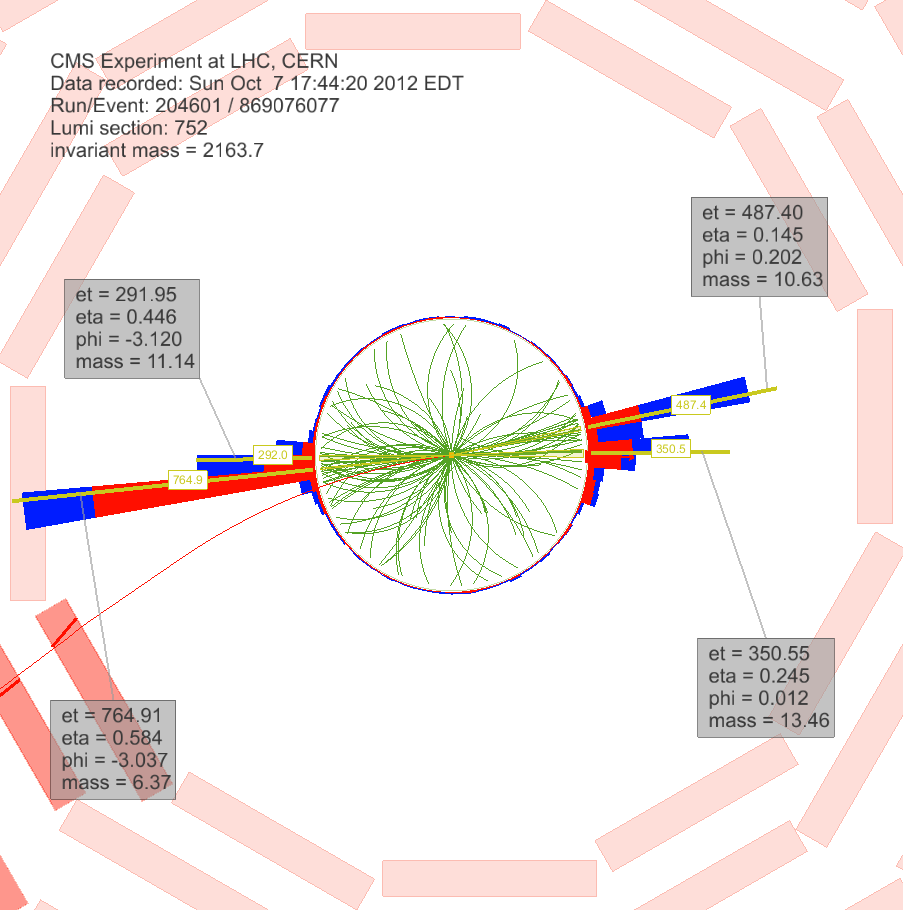
\includegraphics[width=0.6\textwidth,angle=0]{EXO-12-024/figs/event-display/highdoublemass/rho-phi-white.png}
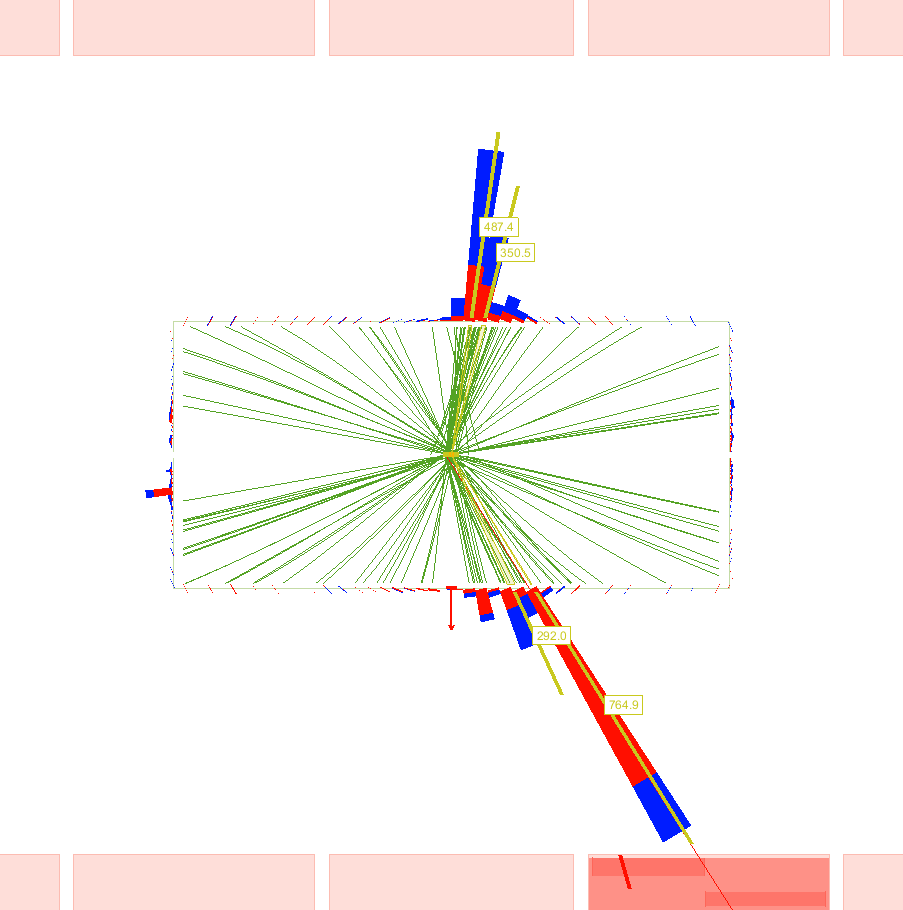
\includegraphics[width=0.6\textwidth,angle=0]{EXO-12-024/figs/event-display/highdoublemass/rho-z-white.png}
\end{center}
\caption{Event display of double W/Z-tagged event with the highest dijet invariant mass of 2.16~\TeVcc .
The transverse momenta of the two leading jets are 1.1~\TeVcc and 0.92~\TeVcc .
The invariant mass of the two leading pruned CA8 jets is 97.82 \GeVcc and 85.08 \GeVcc .
}
\label{fig:eventdisplay1}
\end{figure}

\begin{figure}[!htbp]
\begin{center}
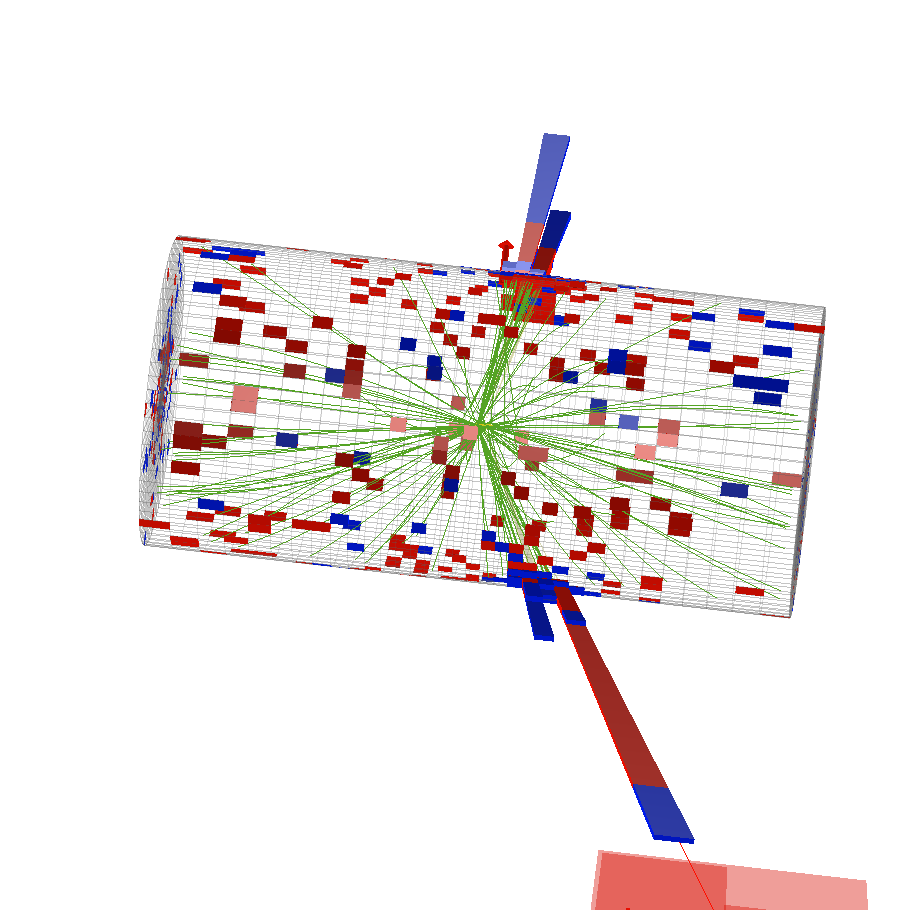
\includegraphics[width=0.6\textwidth,angle=0]{EXO-12-024/figs/event-display/highdoublemass/tower-white.png}
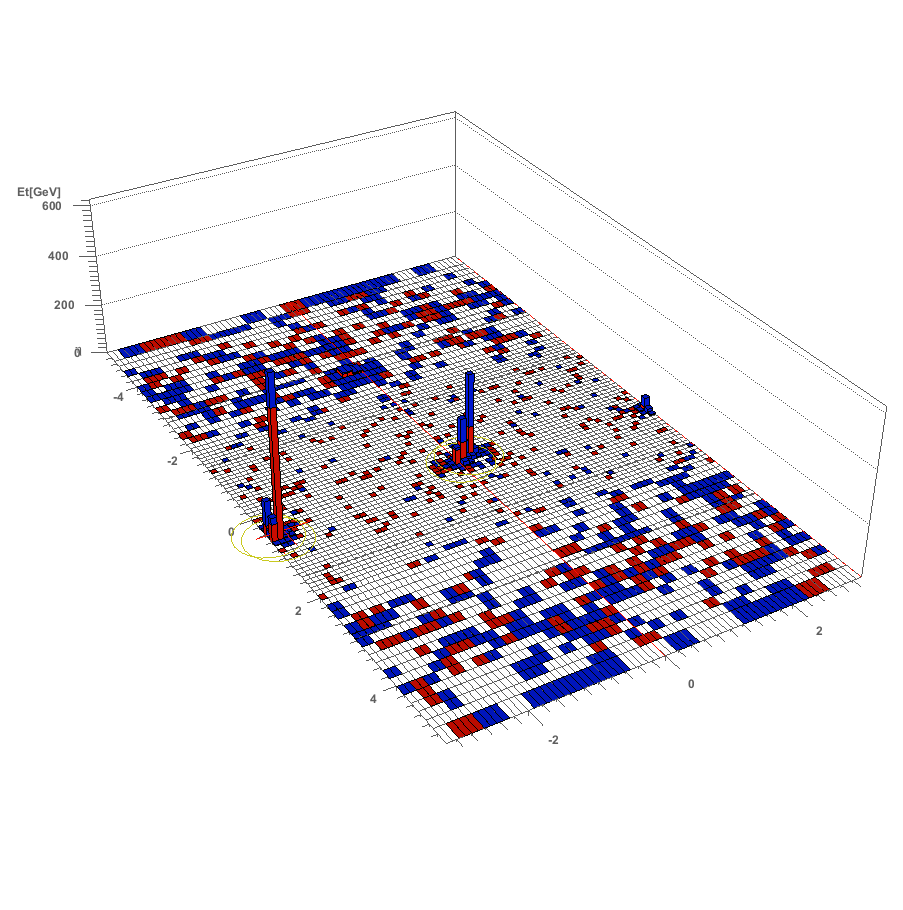
\includegraphics[width=0.6\textwidth,angle=0]{EXO-12-024/figs/event-display/highdoublemass/lego-white.png}
\end{center}
\caption{Event display of double W/Z-tagged event with the highest dijet invariant mass of 2.16~\TeVcc .
The transverse momenta of the two leading jets are 1.1~\TeVcc and 0.92~\TeVcc .
The invariant mass of the two leading pruned CA8 jets is 97.82 \GeVcc and 85.08 \GeVcc .
}
\label{fig:eventdisplay2}
\end{figure}


\subsection{Jet reconstruction}

\label{sec:reconstruction}


Based on CMSSW 5.3.x software package,events are reconstructed using the particle-flow reconstruction
algorithm~\cite{particleflow}, which attempts to reconstruct all
stable particles in an event by combining information from all
subdetectors. The algorithm categorizes all particles into five types:
muons, electrons, photons, charged and neutral hadrons. The resulting
particle flow candidates are passed to each jet clustering algorithm, in this case the
Cambridge-Aachen (CA)~\cite{CAaachen,CAcambridge}
jet clustering algorithm, as implemented in FastJet version 3.0.1 \cite{fastjet1,fastjet},
to create "particle flow jets".
The CA clustering sequence is only determined by the distance between
clusters and is not weighted by their momentum, as is done for the
$k_\text{T}$ and anti-$k_\text{T}$ algorithms. A distance parameter of
size $R=\sqrt{(\Delta \eta)^2 + (\Delta\phi)^2}=0.8$ is used for the CA algorithm.
%In previous studies based on simulation~\cite{catop_cms}, the CA algorithm was
%found to be more efficient (for the same mistag rate) than $k_{\mathrm  T}$
%or anti-$k_{\mathrm T}$ at finding hard subjets by reversing
%the last step of the clustering algorithm.


Charged hadrons identified as pileup are removed from the inputs to
the jet clustering algorithms.  The remaining neutral component of pileup
is removed by applying a residual area-based correction as
described in Ref.~\cite{jetarea_fastjet,jetarea_fastjet_pu}.  The mean
$\pt$ per unit area is computed with the $k_{\mathrm T}$ algorithm
with the ``active area'' method, with a distance parameter of 0.6, and
the jet energy is corrected by the amount of pileup expected in the
jet area. The amount of energy expected from the underlying event is
added back into the jet.  The pileup-subtracted jet four momenta are
finally corrected for nonlinearities in $\eta$ and $\pt$ with
simulated data, with a residual $\eta$-dependent correction added to
correct for the difference in simulated and true
responses~\cite{JME-JINST,Collaboration:2012dp}.

The jet energy corrections for the CA $R=0.8$ jets are derived from studies using the
anti-$k_{\mathrm T}$ $R=0.7$ jet algorithm. Simulation studies confirm that these
anti-$k_{\mathrm T}$-derived jet corrections
are adequate for the CA $R=0.8$ jet algorithm for the jet momenta
considered here~\cite{topwtag_pas}.% within an additional uncertainty of 2\%.


\subsection{Event selection}
\label{event_selection}

Events are selected using the following cuts:
\begin{itemize}
\item The event must have a well reconstructed primary vertex as computed by a deterministic annealing filter (DAF)
($\vert z_\text{Primary Vertex}\vert < 24$ cm, $N_\text{DOF} > 6$).
\item The following recommended noise event filters are used:
       \begin{itemize}
          \item  CSC tight beam halo filter
          \item  HBHE noise filter with isolated noise rejection
          \item  HCAL laser event filter (HBHE) and HCAL laser event filter 2012
          \item  ECAL dead cell trigger primitive (TP) filter
          \item  The beam scraping filter
          \item  Bad EE supercrystal filter
          \item  The tracking failure filter
          \item  Good primary vertex filter 
	  \item  Tracking coherent noise filter
	  \item  Tracking TOBTEC fakes filter  
       \end{itemize}
\item The events are required to have at least two ungroomed CA8 jets with
        \begin{itemize}
          \item $\pt > 30$ \GeVcc, $|\eta| < 2.5$
          \item  to have muon energy fraction $< 0.8$
          \item pass tight particle flow jet ID. The tight PF jet ID is listed below:
                 \begin{itemize}
                     \item   Neutral Hadron (EM) Fraction $< 0.90 (< 0.90)$, for all jet $\eta$
                     \item   Number of Constituents $> 1$, for all jet $\eta$
                     \item   Charged Hadron (EM) Fraction $> 0 (< 0.99)$, for jet $|\eta| < 2.4$
                     \item   Charged Multiplicity$ > 0$, for jet $|\eta| < 2.4$
                 \end{itemize}
        \end{itemize}
\item Beam background events are removed using the following requirements:
        \begin{itemize}
        \item In events with at least 10 tracks, a minimum of 25\% of
          these tracks must be high purity tracks.
        \end{itemize}
\item  We also require $E_{T}^{miss}/\sum{E_{T}} < 0.5$ to further suppress the noise producing large fake $E_{T}^{miss}$. 
\item The events must pass $|\Delta\eta|<1.3$, $m_{jj} > 890  \GeVcc$
\end{itemize}

This sample of dijet events is then tested for presence of
hadronically decaying W or Z bosons.
